\documentclass[a4paper]{book}
\usepackage{a4wide}
\usepackage{makeidx}
\usepackage{graphicx}
\usepackage{multicol}
\usepackage{float}
\usepackage{listings}
\usepackage{color}
\usepackage{textcomp}
\usepackage{alltt}
\usepackage{times}
\usepackage{ifpdf}
\ifpdf
\usepackage[pdftex,
            pagebackref=true,
            colorlinks=true,
            linkcolor=blue,
            unicode
           ]{hyperref}
\else
\usepackage[ps2pdf,
            pagebackref=true,
            colorlinks=true,
            linkcolor=blue,
            unicode
           ]{hyperref}
\usepackage{pspicture}
\fi
\usepackage[utf8]{inputenc}
\usepackage{doxygen}
\lstset{language=C++,inputencoding=utf8,basicstyle=\footnotesize,breaklines=true,breakatwhitespace=true,tabsize=8,numbers=left }
\makeindex
\setcounter{tocdepth}{3}
\renewcommand{\footrulewidth}{0.4pt}
\begin{document}
\hypersetup{pageanchor=false}
\begin{titlepage}
\vspace*{7cm}
\begin{center}
{\Large PolyUnpack }\\
\vspace*{1cm}
{\large Generated by Doxygen 1.6.3}\\
\vspace*{0.5cm}
{\small Sun May 13 02:22:33 2012}\\
\end{center}
\end{titlepage}
\clearemptydoublepage
\pagenumbering{roman}
\tableofcontents
\clearemptydoublepage
\pagenumbering{arabic}
\hypersetup{pageanchor=true}
\chapter{Description}
\label{index}\hypertarget{index}{}The program is implementation of the algorithm proposed by Paul Royal, Mitch Halpin, etc. in the article \char`\"{}PolyUnpack: Automating the Hidden-\/Code
Extraction of Unpack-\/Executing Malware\char`\"{} in 2006. They describe a method for detecting self-\/decrypting exploit codes. It scans network traffic and uses static analysis and emulated instruction execution techniques. The program works as a console utility. \begin{DoxyAuthor}{Author}
Platonov Ivan \href{mailto:platonovmsu@gmail.com}{\tt platonovmsu@gmail.com} 
\end{DoxyAuthor}

\chapter{Class Index}
\section{Class Hierarchy}
This inheritance list is sorted roughly, but not completely, alphabetically:\begin{DoxyCompactList}
\item \contentsline{section}{contains}{\pageref{classcontains}}{}
\item \contentsline{section}{emulates}{\pageref{classemulates}}{}
\item \contentsline{section}{Emulator\_\-LibEmu}{\pageref{classEmulator__LibEmu}}{}
\item \contentsline{section}{In}{\pageref{classIn}}{}
\item \contentsline{section}{Instruction\_\-Leaf}{\pageref{structInstruction__Leaf}}{}
\item \contentsline{section}{Instruction\_\-Tree}{\pageref{classInstruction__Tree}}{}
\item \contentsline{section}{InstructionList}{\pageref{structInstructionList}}{}
\item \contentsline{section}{List\_\-of\_\-Return\_\-Addresses}{\pageref{structList__of__Return__Addresses}}{}
\item \contentsline{section}{PolyUnpack}{\pageref{classPolyUnpack}}{}
\item \contentsline{section}{Reader}{\pageref{classReader}}{}
\begin{DoxyCompactList}
\item \contentsline{section}{PE\_\-Reader}{\pageref{classPE__Reader}}{}
\item \contentsline{section}{Raw\_\-Reader}{\pageref{classRaw__Reader}}{}
\end{DoxyCompactList}
\item \contentsline{section}{Stack}{\pageref{classStack}}{}
\item \contentsline{section}{Used}{\pageref{structUsed}}{}
\end{DoxyCompactList}

\chapter{Class Index}
\section{Class List}
Here are the classes, structs, unions and interfaces with brief descriptions:\begin{DoxyCompactList}
\item\contentsline{section}{\hyperlink{classcontains}{contains} }{\pageref{classcontains}}{}
\item\contentsline{section}{\hyperlink{classemulates}{emulates} }{\pageref{classemulates}}{}
\item\contentsline{section}{\hyperlink{classEmulator__LibEmu}{Emulator\_\-LibEmu} }{\pageref{classEmulator__LibEmu}}{}
\item\contentsline{section}{\hyperlink{classIn}{In} }{\pageref{classIn}}{}
\item\contentsline{section}{\hyperlink{structInstruction__Leaf}{Instruction\_\-Leaf} }{\pageref{structInstruction__Leaf}}{}
\item\contentsline{section}{\hyperlink{classInstruction__Tree}{Instruction\_\-Tree} }{\pageref{classInstruction__Tree}}{}
\item\contentsline{section}{\hyperlink{structInstructionList}{InstructionList} }{\pageref{structInstructionList}}{}
\item\contentsline{section}{\hyperlink{structList__of__Return__Addresses}{List\_\-of\_\-Return\_\-Addresses} }{\pageref{structList__of__Return__Addresses}}{}
\item\contentsline{section}{\hyperlink{classPE__Reader}{PE\_\-Reader} }{\pageref{classPE__Reader}}{}
\item\contentsline{section}{\hyperlink{classPolyUnpack}{PolyUnpack} }{\pageref{classPolyUnpack}}{}
\item\contentsline{section}{\hyperlink{classRaw__Reader}{Raw\_\-Reader} }{\pageref{classRaw__Reader}}{}
\item\contentsline{section}{\hyperlink{classReader}{Reader} }{\pageref{classReader}}{}
\item\contentsline{section}{\hyperlink{classStack}{Stack} }{\pageref{classStack}}{}
\item\contentsline{section}{\hyperlink{structUsed}{Used} }{\pageref{structUsed}}{}
\end{DoxyCompactList}

\chapter{Class Documentation}
\hypertarget{classcontains}{
\section{contains Class Reference}
\label{classcontains}\index{contains@{contains}}
}


\subsection{Detailed Description}
logic of the algorithm 

The documentation for this class was generated from the following file:\begin{DoxyCompactItemize}
\item 
PolyUnpack.h\end{DoxyCompactItemize}

\hypertarget{classemulates}{
\section{emulates Class Reference}
\label{classemulates}\index{emulates@{emulates}}
}


\subsection{Detailed Description}
step. 

The documentation for this class was generated from the following file:\begin{DoxyCompactItemize}
\item 
Emulator\_\-LibEmu.h\end{DoxyCompactItemize}

\hypertarget{classEmulator__LibEmu}{
\section{Emulator\_\-LibEmu Class Reference}
\label{classEmulator__LibEmu}\index{Emulator\_\-LibEmu@{Emulator\_\-LibEmu}}
}
\subsection*{Public Member Functions}
\begin{DoxyCompactItemize}
\item 
\hyperlink{classEmulator__LibEmu_ae8595b6312f2125ed061293d689ff23c}{Emulator\_\-LibEmu} ()
\begin{DoxyCompactList}\small\item\em image base (from what address we need to load file for emulation) \item\end{DoxyCompactList}\item 
\hyperlink{classEmulator__LibEmu_a358ea52a971cbb5e14b6e08bcbaa29fb}{$\sim$Emulator\_\-LibEmu} ()
\item 
void \hyperlink{classEmulator__LibEmu_af64acac5abd8f8c2e48ea8ac8e6a3a28}{begin} (char $\ast$\&buf, const unsigned int len, const unsigned int entry\_\-point, const unsigned int base)
\item 
void \hyperlink{classEmulator__LibEmu_a998a8239af4107121592764094de152c}{jump} (const unsigned int pos)
\item 
bool \hyperlink{classEmulator__LibEmu_a2d1424d0a52e51b37788e6186cc1ba9f}{step} ()
\item 
void \hyperlink{classEmulator__LibEmu_a8779c16bb5b588252c0d2d048c7954c5}{get\_\-command} (char $\ast$buf, const unsigned int size) const 
\item 
void \hyperlink{classEmulator__LibEmu_ab0b54d3e5a0b42ab48da798dc49b3306}{read\_\-block} (char $\ast$buf, const unsigned int size) const 
\item 
unsigned int \hyperlink{classEmulator__LibEmu_a574c79f85662bee6c54bf32f0203baf5}{get\_\-register} (const Register reg) const 
\item 
unsigned int \hyperlink{classEmulator__LibEmu_ad6f5f9fcfa552bf5865b6c9a432aa2ba}{get\_\-register} (char $\ast$\&string) const 
\end{DoxyCompactItemize}


\subsection{Constructor \& Destructor Documentation}
\hypertarget{classEmulator__LibEmu_ae8595b6312f2125ed061293d689ff23c}{
\index{Emulator\_\-LibEmu@{Emulator\_\-LibEmu}!Emulator\_\-LibEmu@{Emulator\_\-LibEmu}}
\index{Emulator\_\-LibEmu@{Emulator\_\-LibEmu}!Emulator_LibEmu@{Emulator\_\-LibEmu}}
\subsubsection[{Emulator\_\-LibEmu}]{\setlength{\rightskip}{0pt plus 5cm}Emulator\_\-LibEmu::Emulator\_\-LibEmu ()}}
\label{classEmulator__LibEmu_ae8595b6312f2125ed061293d689ff23c}


image base (from what address we need to load file for emulation) 

Constructor \hypertarget{classEmulator__LibEmu_a358ea52a971cbb5e14b6e08bcbaa29fb}{
\index{Emulator\_\-LibEmu@{Emulator\_\-LibEmu}!$\sim$Emulator\_\-LibEmu@{$\sim$Emulator\_\-LibEmu}}
\index{$\sim$Emulator\_\-LibEmu@{$\sim$Emulator\_\-LibEmu}!Emulator_LibEmu@{Emulator\_\-LibEmu}}
\subsubsection[{$\sim$Emulator\_\-LibEmu}]{\setlength{\rightskip}{0pt plus 5cm}Emulator\_\-LibEmu::$\sim$Emulator\_\-LibEmu ()}}
\label{classEmulator__LibEmu_a358ea52a971cbb5e14b6e08bcbaa29fb}
Destructor 

\subsection{Member Function Documentation}
\hypertarget{classEmulator__LibEmu_af64acac5abd8f8c2e48ea8ac8e6a3a28}{
\index{Emulator\_\-LibEmu@{Emulator\_\-LibEmu}!begin@{begin}}
\index{begin@{begin}!Emulator_LibEmu@{Emulator\_\-LibEmu}}
\subsubsection[{begin}]{\setlength{\rightskip}{0pt plus 5cm}void Emulator\_\-LibEmu::begin (char $\ast$\& {\em buf}, \/  const unsigned int {\em len}, \/  const unsigned int {\em entry\_\-point}, \/  const unsigned int {\em base})}}
\label{classEmulator__LibEmu_af64acac5abd8f8c2e48ea8ac8e6a3a28}
Loads file in emulator memory, sets all registers in 0 and sets eip to the entry point 
\begin{DoxyParams}{Parameters}
\item[{\em buf}]buffer \item[{\em len}]buffer size \item[{\em entry\_\-point}]entry point \item[{\em base}]image base \end{DoxyParams}
\hypertarget{classEmulator__LibEmu_a8779c16bb5b588252c0d2d048c7954c5}{
\index{Emulator\_\-LibEmu@{Emulator\_\-LibEmu}!get\_\-command@{get\_\-command}}
\index{get\_\-command@{get\_\-command}!Emulator_LibEmu@{Emulator\_\-LibEmu}}
\subsubsection[{get\_\-command}]{\setlength{\rightskip}{0pt plus 5cm}void Emulator\_\-LibEmu::get\_\-command (char $\ast$ {\em buf}, \/  const unsigned int {\em size}) const}}
\label{classEmulator__LibEmu_a8779c16bb5b588252c0d2d048c7954c5}
Reads size bytes into the buffer from emulator memory 
\begin{DoxyParams}{Parameters}
\item[{\em buf}]buffer where to read \item[{\em size}]size of buffer \end{DoxyParams}
\hypertarget{classEmulator__LibEmu_ad6f5f9fcfa552bf5865b6c9a432aa2ba}{
\index{Emulator\_\-LibEmu@{Emulator\_\-LibEmu}!get\_\-register@{get\_\-register}}
\index{get\_\-register@{get\_\-register}!Emulator_LibEmu@{Emulator\_\-LibEmu}}
\subsubsection[{get\_\-register}]{\setlength{\rightskip}{0pt plus 5cm}unsigned int Emulator\_\-LibEmu::get\_\-register (char $\ast$\& {\em string}) const}}
\label{classEmulator__LibEmu_ad6f5f9fcfa552bf5865b6c9a432aa2ba}
Gets value of register 
\begin{DoxyParams}{Parameters}
\item[{\em string}]string with register name \end{DoxyParams}
\begin{DoxyReturn}{Returns}
value 
\end{DoxyReturn}
\hypertarget{classEmulator__LibEmu_a574c79f85662bee6c54bf32f0203baf5}{
\index{Emulator\_\-LibEmu@{Emulator\_\-LibEmu}!get\_\-register@{get\_\-register}}
\index{get\_\-register@{get\_\-register}!Emulator_LibEmu@{Emulator\_\-LibEmu}}
\subsubsection[{get\_\-register}]{\setlength{\rightskip}{0pt plus 5cm}unsigned int Emulator\_\-LibEmu::get\_\-register (const Register {\em reg}) const}}
\label{classEmulator__LibEmu_a574c79f85662bee6c54bf32f0203baf5}
Gets value of register reg 
\begin{DoxyParams}{Parameters}
\item[{\em reg}]register \end{DoxyParams}
\begin{DoxyReturn}{Returns}
value 
\end{DoxyReturn}
\hypertarget{classEmulator__LibEmu_a998a8239af4107121592764094de152c}{
\index{Emulator\_\-LibEmu@{Emulator\_\-LibEmu}!jump@{jump}}
\index{jump@{jump}!Emulator_LibEmu@{Emulator\_\-LibEmu}}
\subsubsection[{jump}]{\setlength{\rightskip}{0pt plus 5cm}void Emulator\_\-LibEmu::jump (const unsigned int {\em pos})}}
\label{classEmulator__LibEmu_a998a8239af4107121592764094de152c}
Sets eip to the nesessary address 
\begin{DoxyParams}{Parameters}
\item[{\em pos}]address \end{DoxyParams}
\hypertarget{classEmulator__LibEmu_ab0b54d3e5a0b42ab48da798dc49b3306}{
\index{Emulator\_\-LibEmu@{Emulator\_\-LibEmu}!read\_\-block@{read\_\-block}}
\index{read\_\-block@{read\_\-block}!Emulator_LibEmu@{Emulator\_\-LibEmu}}
\subsubsection[{read\_\-block}]{\setlength{\rightskip}{0pt plus 5cm}void Emulator\_\-LibEmu::read\_\-block (char $\ast$ {\em buf}, \/  const unsigned int {\em size}) const}}
\label{classEmulator__LibEmu_ab0b54d3e5a0b42ab48da798dc49b3306}
Helps to work with buffer after emulation 
\begin{DoxyParams}{Parameters}
\item[{\em buf}]buffer \item[{\em size}]size of buffer \end{DoxyParams}
\hypertarget{classEmulator__LibEmu_a2d1424d0a52e51b37788e6186cc1ba9f}{
\index{Emulator\_\-LibEmu@{Emulator\_\-LibEmu}!step@{step}}
\index{step@{step}!Emulator_LibEmu@{Emulator\_\-LibEmu}}
\subsubsection[{step}]{\setlength{\rightskip}{0pt plus 5cm}bool Emulator\_\-LibEmu::step ()}}
\label{classEmulator__LibEmu_a2d1424d0a52e51b37788e6186cc1ba9f}
Emulates execution of one instruction. Calls two functions bool emu\_\-cpu\_\-parse(cpu) and bool emu\_\-cpu\_\-step(cpu). \begin{DoxyReturn}{Returns}
false if one of this functions return false. \hyperlink{classIn}{In} another case returns true. 
\end{DoxyReturn}


The documentation for this class was generated from the following files:\begin{DoxyCompactItemize}
\item 
Emulator\_\-LibEmu.h\item 
Emulator\_\-LibEmu.cpp\end{DoxyCompactItemize}

\hypertarget{classIn}{
\section{In Class Reference}
\label{classIn}\index{In@{In}}
}


\subsection{Detailed Description}
execution it needs to find the right way in case of condition jump. So that we can compare instructions properly. For this target \hyperlink{classInstruction__Tree}{Instruction\_\-Tree} is used. It helps to control any possible variants of execution. It is a bit difficult to understand logic of members of this class. If you have any problems, please contact me. I will be glad to explain it. 

The documentation for this class was generated from the following file:\begin{DoxyCompactItemize}
\item 
PolyUnpack.h\end{DoxyCompactItemize}

\hypertarget{structInstruction__Leaf}{
\section{Instruction\_\-Leaf Struct Reference}
\label{structInstruction__Leaf}\index{Instruction\_\-Leaf@{Instruction\_\-Leaf}}
}
\subsection*{Public Attributes}
\begin{DoxyCompactItemize}
\item 
\hypertarget{structInstruction__Leaf_a3bdd875389a52faec9a2c22e34587e03}{
\hyperlink{structInstructionList}{InstructionList} $\ast$ {\bfseries pointer}}
\label{structInstruction__Leaf_a3bdd875389a52faec9a2c22e34587e03}

\item 
\hypertarget{structInstruction__Leaf_a6b61ac5226219e5ccd91e341682b53c2}{
\hyperlink{structInstruction__Leaf}{Instruction\_\-Leaf} $\ast$ \hyperlink{structInstruction__Leaf_a6b61ac5226219e5ccd91e341682b53c2}{left}}
\label{structInstruction__Leaf_a6b61ac5226219e5ccd91e341682b53c2}

\begin{DoxyCompactList}\small\item\em pointer to struct \hyperlink{structInstructionList}{InstructionList}. So that we can use member char$\ast$ instruction in \hyperlink{structInstructionList}{InstructionList}. \item\end{DoxyCompactList}\item 
\hypertarget{structInstruction__Leaf_a0aaf651c987a0f4b43a147a0f12aa4af}{
\hyperlink{structInstruction__Leaf}{Instruction\_\-Leaf} $\ast$ \hyperlink{structInstruction__Leaf_a0aaf651c987a0f4b43a147a0f12aa4af}{right}}
\label{structInstruction__Leaf_a0aaf651c987a0f4b43a147a0f12aa4af}

\begin{DoxyCompactList}\small\item\em pointer to the left node/leaf in \hyperlink{classInstruction__Tree}{Instruction\_\-Tree}. If it is leaf then left=NULL. \item\end{DoxyCompactList}\item 
\hypertarget{structInstruction__Leaf_ac32816e6c74234c4bcb8f3442a387bf2}{
int \hyperlink{structInstruction__Leaf_ac32816e6c74234c4bcb8f3442a387bf2}{valid}}
\label{structInstruction__Leaf_ac32816e6c74234c4bcb8f3442a387bf2}

\begin{DoxyCompactList}\small\item\em pointer to the right node/leaf in \hyperlink{classInstruction__Tree}{Instruction\_\-Tree}. If it is leaf then right=NULL. \item\end{DoxyCompactList}\end{DoxyCompactItemize}


The documentation for this struct was generated from the following file:\begin{DoxyCompactItemize}
\item 
Instruction\_\-Leaf.h\end{DoxyCompactItemize}

\hypertarget{classInstruction__Tree}{
\section{Instruction\_\-Tree Class Reference}
\label{classInstruction__Tree}\index{Instruction\_\-Tree@{Instruction\_\-Tree}}
}
\subsection*{Public Member Functions}
\begin{DoxyCompactItemize}
\item 
\hypertarget{classInstruction__Tree_af6984c818a0944ed8d4b2d0b9d9ec6d6}{
void {\bfseries Add} (\hyperlink{structInstructionList}{InstructionList} $\ast$\&, \hyperlink{structInstructionList}{InstructionList} $\ast$\&, \hyperlink{structInstructionList}{InstructionList} $\ast$\&)}
\label{classInstruction__Tree_af6984c818a0944ed8d4b2d0b9d9ec6d6}

\item 
\hypertarget{classInstruction__Tree_aad648a9a8074aeafbf78e9c828afd048}{
void {\bfseries Add\_\-Leaf} (\hyperlink{structInstruction__Leaf}{Instruction\_\-Leaf} $\ast$\&, int, \hyperlink{structInstructionList}{InstructionList} $\ast$\&, \hyperlink{structInstructionList}{InstructionList} $\ast$\&)}
\label{classInstruction__Tree_aad648a9a8074aeafbf78e9c828afd048}

\item 
\hypertarget{classInstruction__Tree_a226966bee997b0565500106dc2e567d2}{
int {\bfseries Obhod} (const char $\ast$, \hyperlink{classPolyUnpack}{PolyUnpack} \&)}
\label{classInstruction__Tree_a226966bee997b0565500106dc2e567d2}

\item 
\hypertarget{classInstruction__Tree_acedea0a0f4812fe9ce27cac32d69c479}{
void {\bfseries Obhod} (\hyperlink{structInstruction__Leaf}{Instruction\_\-Leaf} $\ast$\&, const char $\ast$, \hyperlink{structInstructionList}{InstructionList} $\ast$\&, \hyperlink{classPolyUnpack}{PolyUnpack} \&, int \&, int \&, int \&)}
\label{classInstruction__Tree_acedea0a0f4812fe9ce27cac32d69c479}

\item 
\hypertarget{classInstruction__Tree_a1e067a81a558de827a34cc0e302ac5f6}{
void {\bfseries Obhod2} (\hyperlink{structInstruction__Leaf}{Instruction\_\-Leaf} $\ast$\&)}
\label{classInstruction__Tree_a1e067a81a558de827a34cc0e302ac5f6}

\item 
\hypertarget{classInstruction__Tree_a3342c7b010e7760be6034ca09efd97f8}{
int {\bfseries Check} (\hyperlink{structInstruction__Leaf}{Instruction\_\-Leaf} $\ast$\&, \hyperlink{structInstructionList}{InstructionList} $\ast$\&, \hyperlink{structInstructionList}{InstructionList} $\ast$\&, \hyperlink{structInstructionList}{InstructionList} $\ast$\&, \hyperlink{structInstructionList}{InstructionList} $\ast$\&, bool \&flag)}
\label{classInstruction__Tree_a3342c7b010e7760be6034ca09efd97f8}

\item 
\hypertarget{classInstruction__Tree_accb3231bdc3392cc49a8f6b6c79c82a1}{
bool {\bfseries Is\_\-Empty} ()}
\label{classInstruction__Tree_accb3231bdc3392cc49a8f6b6c79c82a1}

\item 
\hypertarget{classInstruction__Tree_aec22cabc78f01e5e543ddb0e6b15be56}{
void {\bfseries Destructor} (\hyperlink{structInstruction__Leaf}{Instruction\_\-Leaf} $\ast$\&)}
\label{classInstruction__Tree_aec22cabc78f01e5e543ddb0e6b15be56}

\item 
\hypertarget{classInstruction__Tree_ad53b5fae2cc7e47a3ec905eade35c8ae}{
void {\bfseries CopyCommand} (\hyperlink{structInstruction__Leaf}{Instruction\_\-Leaf} $\ast$\&, const char $\ast$str)}
\label{classInstruction__Tree_ad53b5fae2cc7e47a3ec905eade35c8ae}

\item 
\hyperlink{classInstruction__Tree_a5d61b36f6c10b48c4ec6d844226a81eb}{Instruction\_\-Tree} ()
\begin{DoxyCompactList}\small\item\em root of the tree. Contains some condition jump command \item\end{DoxyCompactList}\item 
void \hyperlink{classInstruction__Tree_a4c51fc44c6c0fd0d145900231fa1f059}{Add} (\hyperlink{structInstructionList}{InstructionList} $\ast$\&po1, \hyperlink{structInstructionList}{InstructionList} $\ast$\&po2, \hyperlink{structInstructionList}{InstructionList} $\ast$\&po3)
\item 
int \hyperlink{classInstruction__Tree_adef0585fdc4173cbd6baabd5bec79a56}{Obhod} (const char $\ast$command, \hyperlink{classPolyUnpack}{PolyUnpack} \&unpack)
\item 
void \hyperlink{classInstruction__Tree_afc8fc8d76c6ab64eedf78c551972f2df}{Obhod} (\hyperlink{structInstruction__Leaf}{Instruction\_\-Leaf} $\ast$\&p1, const char $\ast$command, \hyperlink{structInstructionList}{InstructionList} $\ast$\&original, \hyperlink{classPolyUnpack}{PolyUnpack} \&unpack, int \&kol, int \&iterator, int \&result)
\item 
void \hyperlink{classInstruction__Tree_ae791340bf25bcf1bf72072d6cc9a5d3e}{Print} (\hyperlink{structInstruction__Leaf}{Instruction\_\-Leaf} $\ast$\&p1)
\item 
int \hyperlink{classInstruction__Tree_ad9da870498b9d71cbb5a720253016712}{Check} (\hyperlink{structInstruction__Leaf}{Instruction\_\-Leaf} $\ast$\&p1, \hyperlink{structInstructionList}{InstructionList} $\ast$\&po1, \hyperlink{structInstructionList}{InstructionList} $\ast$\&po2, \hyperlink{structInstructionList}{InstructionList} $\ast$\&po3, \hyperlink{structInstructionList}{InstructionList} $\ast$\&original, bool \&flag)
\item 
bool \hyperlink{classInstruction__Tree_accb3231bdc3392cc49a8f6b6c79c82a1}{Is\_\-Empty} ()
\item 
void \hyperlink{classInstruction__Tree_a3ede055013058a1f9abefb5f50c02423}{Destructor} (\hyperlink{structInstruction__Leaf}{Instruction\_\-Leaf} $\ast$\&p1)
\item 
\hyperlink{classInstruction__Tree_abbd3825561af346def028707498fbd9b}{$\sim$Instruction\_\-Tree} ()
\end{DoxyCompactItemize}


\subsection{Constructor \& Destructor Documentation}
\hypertarget{classInstruction__Tree_a5d61b36f6c10b48c4ec6d844226a81eb}{
\index{Instruction\_\-Tree@{Instruction\_\-Tree}!Instruction\_\-Tree@{Instruction\_\-Tree}}
\index{Instruction\_\-Tree@{Instruction\_\-Tree}!Instruction_Tree@{Instruction\_\-Tree}}
\subsubsection[{Instruction\_\-Tree}]{\setlength{\rightskip}{0pt plus 5cm}Instruction\_\-Tree::Instruction\_\-Tree ()\hspace{0.3cm}{\ttfamily  \mbox{[}inline\mbox{]}}}}
\label{classInstruction__Tree_a5d61b36f6c10b48c4ec6d844226a81eb}


root of the tree. Contains some condition jump command 

Constructor by default \hypertarget{classInstruction__Tree_abbd3825561af346def028707498fbd9b}{
\index{Instruction\_\-Tree@{Instruction\_\-Tree}!$\sim$Instruction\_\-Tree@{$\sim$Instruction\_\-Tree}}
\index{$\sim$Instruction\_\-Tree@{$\sim$Instruction\_\-Tree}!Instruction_Tree@{Instruction\_\-Tree}}
\subsubsection[{$\sim$Instruction\_\-Tree}]{\setlength{\rightskip}{0pt plus 5cm}Instruction\_\-Tree::$\sim$Instruction\_\-Tree ()}}
\label{classInstruction__Tree_abbd3825561af346def028707498fbd9b}
Destructor 

\subsection{Member Function Documentation}
\hypertarget{classInstruction__Tree_a4c51fc44c6c0fd0d145900231fa1f059}{
\index{Instruction\_\-Tree@{Instruction\_\-Tree}!Add@{Add}}
\index{Add@{Add}!Instruction_Tree@{Instruction\_\-Tree}}
\subsubsection[{Add}]{\setlength{\rightskip}{0pt plus 5cm}void Instruction\_\-Tree::Add ({\bf InstructionList} $\ast$\& {\em po1}, \/  {\bf InstructionList} $\ast$\& {\em po2}, \/  {\bf InstructionList} $\ast$\& {\em po3})}}
\label{classInstruction__Tree_a4c51fc44c6c0fd0d145900231fa1f059}
Add condition jump command in root with two possible instructions, which will be executed next, as leafs. 
\begin{DoxyParams}{Parameters}
\item[{\em po1}]condition inctruction \item[{\em po2}]next instruction after condition jump (left leaf) \item[{\em po3}]another instruction (right leaf) \end{DoxyParams}
\hypertarget{classInstruction__Tree_ad9da870498b9d71cbb5a720253016712}{
\index{Instruction\_\-Tree@{Instruction\_\-Tree}!Check@{Check}}
\index{Check@{Check}!Instruction_Tree@{Instruction\_\-Tree}}
\subsubsection[{Check}]{\setlength{\rightskip}{0pt plus 5cm}int Instruction\_\-Tree::Check ({\bf Instruction\_\-Leaf} $\ast$\& {\em p1}, \/  {\bf InstructionList} $\ast$\& {\em po1}, \/  {\bf InstructionList} $\ast$\& {\em po2}, \/  {\bf InstructionList} $\ast$\& {\em po3}, \/  {\bf InstructionList} $\ast$\& {\em original}, \/  bool \& {\em flag})}}
\label{classInstruction__Tree_ad9da870498b9d71cbb5a720253016712}
Sometimes all valid leafs contain the same condition instructrion, as a root. So we have 'loop'. This function checks for this loops and deletes them. This function uses recursion! 
\begin{DoxyParams}{Parameters}
\item[{\em p1}]temporary root \item[{\em po1}]pointer to instruction in original root \item[{\em po2}]pointer to instruction in left leaf under original root \item[{\em po3}]pointer to instruction in right leaf under original root \item[{\em original}]pointer to instruction in original instruction \item[{\em flag}]is true if loop is presented \end{DoxyParams}
\hypertarget{classInstruction__Tree_a3ede055013058a1f9abefb5f50c02423}{
\index{Instruction\_\-Tree@{Instruction\_\-Tree}!Destructor@{Destructor}}
\index{Destructor@{Destructor}!Instruction_Tree@{Instruction\_\-Tree}}
\subsubsection[{Destructor}]{\setlength{\rightskip}{0pt plus 5cm}void Instruction\_\-Tree::Destructor ({\bf Instruction\_\-Leaf} $\ast$\& {\em p1})}}
\label{classInstruction__Tree_a3ede055013058a1f9abefb5f50c02423}
Deletes all tree and makes root NULL. Function uses recursion. 
\begin{DoxyParams}{Parameters}
\item[{\em p1}]temporary root \end{DoxyParams}
\hypertarget{classInstruction__Tree_accb3231bdc3392cc49a8f6b6c79c82a1}{
\index{Instruction\_\-Tree@{Instruction\_\-Tree}!Is\_\-Empty@{Is\_\-Empty}}
\index{Is\_\-Empty@{Is\_\-Empty}!Instruction_Tree@{Instruction\_\-Tree}}
\subsubsection[{Is\_\-Empty}]{\setlength{\rightskip}{0pt plus 5cm}bool Instruction\_\-Tree::Is\_\-Empty ()}}
\label{classInstruction__Tree_accb3231bdc3392cc49a8f6b6c79c82a1}
Checks if root is empty \begin{DoxyReturn}{Returns}
true if NULL, false if is not NULL. 
\end{DoxyReturn}
\hypertarget{classInstruction__Tree_afc8fc8d76c6ab64eedf78c551972f2df}{
\index{Instruction\_\-Tree@{Instruction\_\-Tree}!Obhod@{Obhod}}
\index{Obhod@{Obhod}!Instruction_Tree@{Instruction\_\-Tree}}
\subsubsection[{Obhod}]{\setlength{\rightskip}{0pt plus 5cm}void Instruction\_\-Tree::Obhod ({\bf Instruction\_\-Leaf} $\ast$\& {\em p1}, \/  const char $\ast$ {\em command}, \/  {\bf InstructionList} $\ast$\& {\em original}, \/  {\bf PolyUnpack} \& {\em unpack}, \/  int \& {\em kol}, \/  int \& {\em iterator}, \/  int \& {\em result})}}
\label{classInstruction__Tree_afc8fc8d76c6ab64eedf78c551972f2df}
The search is performed only in legal branches. To do this we compare 'legal' field in every node. If leaf is valid, one or two branches are added to it. This function uses recursion! 
\begin{DoxyParams}{Parameters}
\item[{\em p1}]temporary root \item[{\em command}]\item[{\em original}]pointer to \hyperlink{structInstructionList}{InstructionList} \item[{\em unpack}]\item[{\em kol}]number of valid leafs \item[{\em iterator}]\item[{\em result}]\end{DoxyParams}
\hypertarget{classInstruction__Tree_adef0585fdc4173cbd6baabd5bec79a56}{
\index{Instruction\_\-Tree@{Instruction\_\-Tree}!Obhod@{Obhod}}
\index{Obhod@{Obhod}!Instruction_Tree@{Instruction\_\-Tree}}
\subsubsection[{Obhod}]{\setlength{\rightskip}{0pt plus 5cm}int Instruction\_\-Tree::Obhod (const char $\ast$ {\em command}, \/  {\bf PolyUnpack} \& {\em unpack})}}
\label{classInstruction__Tree_adef0585fdc4173cbd6baabd5bec79a56}
When root is not empty, we need to compare executed instruction with all leaf instructions in the tree and check amount of legal leafs. If there are not any legal instructions or just one, we need to delete tree. 
\begin{DoxyParams}{Parameters}
\item[{\em command}]executed command to compare with \item[{\em unpack}]We need to compare command with leaf and if it is legal to find another possible ways \end{DoxyParams}
\begin{DoxyReturn}{Returns}
0 if there are not any legal instructions, 1 in another case return a number$>$0. 
\end{DoxyReturn}
\hypertarget{classInstruction__Tree_ae791340bf25bcf1bf72072d6cc9a5d3e}{
\index{Instruction\_\-Tree@{Instruction\_\-Tree}!Print@{Print}}
\index{Print@{Print}!Instruction_Tree@{Instruction\_\-Tree}}
\subsubsection[{Print}]{\setlength{\rightskip}{0pt plus 5cm}void Instruction\_\-Tree::Print ({\bf Instruction\_\-Leaf} $\ast$\& {\em p1})}}
\label{classInstruction__Tree_ae791340bf25bcf1bf72072d6cc9a5d3e}
Print all tree 
\begin{DoxyParams}{Parameters}
\item[{\em p1}]temporary root \end{DoxyParams}


The documentation for this class was generated from the following files:\begin{DoxyCompactItemize}
\item 
Instruction\_\-Tree.h\item 
PolyUnpack.h\item 
Instruction\_\-Tree.cpp\item 
PolyUnpack.cpp\end{DoxyCompactItemize}

\hypertarget{structInstructionList}{
\section{InstructionList Struct Reference}
\label{structInstructionList}\index{InstructionList@{InstructionList}}
}


{\ttfamily \#include $<$InstructionList.h$>$}

\subsection*{Public Attributes}
\begin{DoxyCompactItemize}
\item 
\hypertarget{structInstructionList_ac74eea2eaf0809df3b92cf67fe3862ff}{
char $\ast$ {\bfseries instruction}}
\label{structInstructionList_ac74eea2eaf0809df3b92cf67fe3862ff}

\item 
\hypertarget{structInstructionList_af3462c74f4e95d480be0646b2f605741}{
int \hyperlink{structInstructionList_af3462c74f4e95d480be0646b2f605741}{number}}
\label{structInstructionList_af3462c74f4e95d480be0646b2f605741}

\begin{DoxyCompactList}\small\item\em disassembled instruction in INTEL format \item\end{DoxyCompactList}\item 
\hypertarget{structInstructionList_a7bff02db771b53bfef851bf87a7f9c99}{
int \hyperlink{structInstructionList_a7bff02db771b53bfef851bf87a7f9c99}{length}}
\label{structInstructionList_a7bff02db771b53bfef851bf87a7f9c99}

\begin{DoxyCompactList}\small\item\em offset of instruction from text section \item\end{DoxyCompactList}\item 
\hypertarget{structInstructionList_a44050405954e74cdc3a0ee749046fc0f}{
bool \hyperlink{structInstructionList_a44050405954e74cdc3a0ee749046fc0f}{first}}
\label{structInstructionList_a44050405954e74cdc3a0ee749046fc0f}

\begin{DoxyCompactList}\small\item\em length of instruction \item\end{DoxyCompactList}\item 
\hypertarget{structInstructionList_a6ca0299eca2cd0e7770f17ee1c7e7c91}{
bool \hyperlink{structInstructionList_a6ca0299eca2cd0e7770f17ee1c7e7c91}{padding}}
\label{structInstructionList_a6ca0299eca2cd0e7770f17ee1c7e7c91}

\begin{DoxyCompactList}\small\item\em is true is if instruction is entry point, is false in another case \item\end{DoxyCompactList}\item 
\hypertarget{structInstructionList_a675df0f2d0763aebc20a81b10f8b09c6}{
\hyperlink{structInstructionList}{InstructionList} $\ast$ \hyperlink{structInstructionList_a675df0f2d0763aebc20a81b10f8b09c6}{pointer}}
\label{structInstructionList_a675df0f2d0763aebc20a81b10f8b09c6}

\begin{DoxyCompactList}\small\item\em is true is if instruction is padding, is false in another case \item\end{DoxyCompactList}\end{DoxyCompactItemize}


\subsection{Detailed Description}
List of disassembled instructions from Static Analise 

The documentation for this struct was generated from the following file:\begin{DoxyCompactItemize}
\item 
InstructionList.h\end{DoxyCompactItemize}

\hypertarget{structList__of__Return__Addresses}{
\section{List\_\-of\_\-Return\_\-Addresses Class Reference}
\label{structList__of__Return__Addresses}\index{List\_\-of\_\-Return\_\-Addresses@{List\_\-of\_\-Return\_\-Addresses}}
}


{\ttfamily \#include $<$Stack.h$>$}

\subsection*{Public Attributes}
\begin{DoxyCompactItemize}
\item 
\hypertarget{structList__of__Return__Addresses_a95a492f991784ee1bdee88132b649614}{
unsigned int {\bfseries address}}
\label{structList__of__Return__Addresses_a95a492f991784ee1bdee88132b649614}

\item 
\hypertarget{structList__of__Return__Addresses_a476949fa3ea312b5d54e8d9dc2d5dd73}{
\hyperlink{structList__of__Return__Addresses}{List\_\-of\_\-Return\_\-Addresses} $\ast$ \hyperlink{structList__of__Return__Addresses_a476949fa3ea312b5d54e8d9dc2d5dd73}{pointer}}
\label{structList__of__Return__Addresses_a476949fa3ea312b5d54e8d9dc2d5dd73}

\begin{DoxyCompactList}\small\item\em address of the next instruction after call 0xXXXX instruction \item\end{DoxyCompactList}\end{DoxyCompactItemize}


\subsection{Detailed Description}
Stores information about return addresses 

The documentation for this class was generated from the following file:\begin{DoxyCompactItemize}
\item 
Stack.h\end{DoxyCompactItemize}

\hypertarget{classPE__Reader}{
\section{PE\_\-Reader Class Reference}
\label{classPE__Reader}\index{PE\_\-Reader@{PE\_\-Reader}}
}


{\ttfamily \#include $<$PE\_\-Reader.h$>$}

Inheritance diagram for PE\_\-Reader:\begin{figure}[H]
\begin{center}
\leavevmode
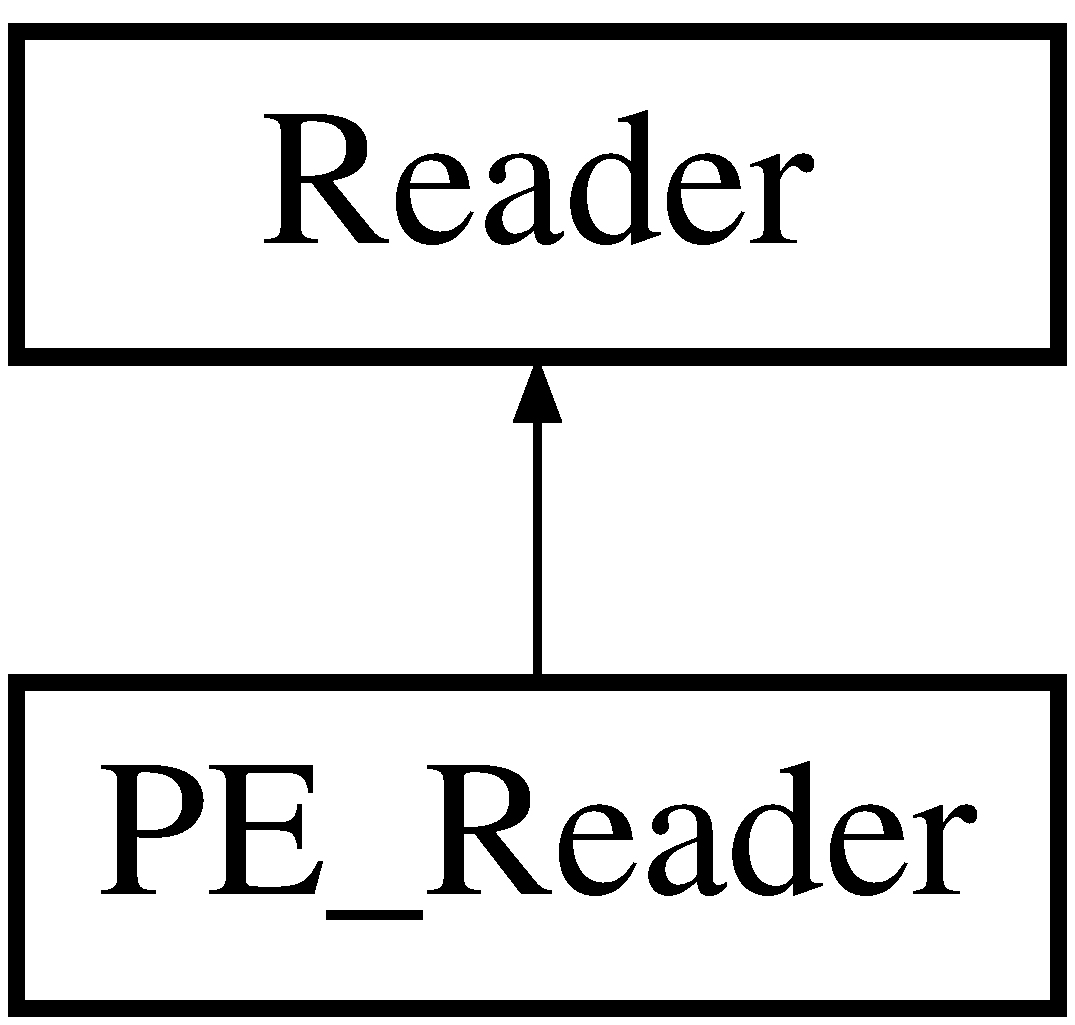
\includegraphics[height=2cm]{classPE__Reader}
\end{center}
\end{figure}
\subsection*{Public Member Functions}
\begin{DoxyCompactItemize}
\item 
\hyperlink{classPE__Reader_a3ee3c529ba07e5cfe8d288fa3ebfa4f9}{PE\_\-Reader} (const char $\ast$name)
\begin{DoxyCompactList}\small\item\em rva address of text sectioon \item\end{DoxyCompactList}\item 
\hyperlink{classPE__Reader_a49781859b63b5d08f49e306f62fc103d}{PE\_\-Reader} (const \hyperlink{classPE__Reader}{PE\_\-Reader} $\ast$pe\_\-reader)
\item 
virtual \hyperlink{classPE__Reader_a6fbfdcd447011a83ac2147874c8e8b4a}{$\sim$PE\_\-Reader} ()
\item 
virtual void \hyperlink{classPE__Reader_a4b5e1c738c887247181c4e3d0f253c27}{LoadForStaticAnalise} (char $\ast$\&buf, unsigned int \&len, unsigned int \&start)
\item 
virtual void \hyperlink{classPE__Reader_ad11f69fdbf231385c9ff7edd26913af7}{LoadForDynamicAnalise} (char $\ast$\&buf, unsigned int \&len, unsigned int \&start, unsigned int \&base, unsigned int \&offset)
\item 
void \hyperlink{classPE__Reader_a6d3abab07f8d39fd1414cad8efb06418}{PE\_\-HeaderOffset} ()
\item 
void \hyperlink{classPE__Reader_a32781a8fee1c88e2ec864ffd1657a192}{PE\_\-TableOffset} ()
\item 
void \hyperlink{classPE__Reader_a492ea400cbf11105f029faab31d0f3fa}{PE\_\-FileType} () const 
\item 
void \hyperlink{classPE__Reader_a6263cdcff862839e6fbbd296c0e060e8}{PE\_\-NumberOfEntries} ()
\item 
void \hyperlink{classPE__Reader_a37d6bf9d6e462f964d77115e29c22418}{PE\_\-EntryPoint} ()
\item 
void \hyperlink{classPE__Reader_a1f263c2df5da0e49bb5211617ae10335}{PE\_\-ImageBase} ()
\item 
void \hyperlink{classPE__Reader_a4896824d5df4cff3d693367fd8d8d454}{PE\_\-ObjectTable} ()
\item 
void \hyperlink{classPE__Reader_a70cf8c6c789cc8c5c96a2b9179043a24}{PE\_\-CodeSection} (int section\_\-offset)
\item 
void \hyperlink{classPE__Reader_a8303dc43c8732907ea8eff507728262b}{PE\_\-DataSection} (int data\_\-offset)
\end{DoxyCompactItemize}


\subsection{Detailed Description}
\hyperlink{classReader}{Reader} for Portable Executable format 

\subsection{Constructor \& Destructor Documentation}
\hypertarget{classPE__Reader_a3ee3c529ba07e5cfe8d288fa3ebfa4f9}{
\index{PE\_\-Reader@{PE\_\-Reader}!PE\_\-Reader@{PE\_\-Reader}}
\index{PE\_\-Reader@{PE\_\-Reader}!PE_Reader@{PE\_\-Reader}}
\subsubsection[{PE\_\-Reader}]{\setlength{\rightskip}{0pt plus 5cm}PE\_\-Reader::PE\_\-Reader (const char $\ast$ {\em name})}}
\label{classPE__Reader_a3ee3c529ba07e5cfe8d288fa3ebfa4f9}


rva address of text sectioon 

Constructor 
\begin{DoxyParams}{Parameters}
\item[{\em name}]file name \end{DoxyParams}
\hypertarget{classPE__Reader_a49781859b63b5d08f49e306f62fc103d}{
\index{PE\_\-Reader@{PE\_\-Reader}!PE\_\-Reader@{PE\_\-Reader}}
\index{PE\_\-Reader@{PE\_\-Reader}!PE_Reader@{PE\_\-Reader}}
\subsubsection[{PE\_\-Reader}]{\setlength{\rightskip}{0pt plus 5cm}PE\_\-Reader::PE\_\-Reader (const {\bf PE\_\-Reader} $\ast$ {\em pe\_\-reader})}}
\label{classPE__Reader_a49781859b63b5d08f49e306f62fc103d}
Copy Constructor 
\begin{DoxyParams}{Parameters}
\item[{\em pe\_\-reader}]\end{DoxyParams}
\hypertarget{classPE__Reader_a6fbfdcd447011a83ac2147874c8e8b4a}{
\index{PE\_\-Reader@{PE\_\-Reader}!$\sim$PE\_\-Reader@{$\sim$PE\_\-Reader}}
\index{$\sim$PE\_\-Reader@{$\sim$PE\_\-Reader}!PE_Reader@{PE\_\-Reader}}
\subsubsection[{$\sim$PE\_\-Reader}]{\setlength{\rightskip}{0pt plus 5cm}PE\_\-Reader::$\sim$PE\_\-Reader ()\hspace{0.3cm}{\ttfamily  \mbox{[}virtual\mbox{]}}}}
\label{classPE__Reader_a6fbfdcd447011a83ac2147874c8e8b4a}
Destructor 

\subsection{Member Function Documentation}
\hypertarget{classPE__Reader_ad11f69fdbf231385c9ff7edd26913af7}{
\index{PE\_\-Reader@{PE\_\-Reader}!LoadForDynamicAnalise@{LoadForDynamicAnalise}}
\index{LoadForDynamicAnalise@{LoadForDynamicAnalise}!PE_Reader@{PE\_\-Reader}}
\subsubsection[{LoadForDynamicAnalise}]{\setlength{\rightskip}{0pt plus 5cm}void PE\_\-Reader::LoadForDynamicAnalise (char $\ast$\& {\em buf}, \/  unsigned int \& {\em len}, \/  unsigned int \& {\em start}, \/  unsigned int \& {\em base}, \/  unsigned int \& {\em offset})\hspace{0.3cm}{\ttfamily  \mbox{[}virtual\mbox{]}}}}
\label{classPE__Reader_ad11f69fdbf231385c9ff7edd26913af7}
Load entire file for Dynamic Analise 
\begin{DoxyParams}{Parameters}
\item[{\em buf}]buffer \item[{\em len}]size of buffer \item[{\em start}]physical original entry point offset \item[{\em base}]is 0x20000000L \item[{\em offset}]physical text section offset \end{DoxyParams}


Implements \hyperlink{classReader_a0fe4ac206880263e042c5277370c679b}{Reader}.

\hypertarget{classPE__Reader_a4b5e1c738c887247181c4e3d0f253c27}{
\index{PE\_\-Reader@{PE\_\-Reader}!LoadForStaticAnalise@{LoadForStaticAnalise}}
\index{LoadForStaticAnalise@{LoadForStaticAnalise}!PE_Reader@{PE\_\-Reader}}
\subsubsection[{LoadForStaticAnalise}]{\setlength{\rightskip}{0pt plus 5cm}void PE\_\-Reader::LoadForStaticAnalise (char $\ast$\& {\em buf}, \/  unsigned int \& {\em len}, \/  unsigned int \& {\em start})\hspace{0.3cm}{\ttfamily  \mbox{[}virtual\mbox{]}}}}
\label{classPE__Reader_a4b5e1c738c887247181c4e3d0f253c27}
Load .text section for Static Analise 
\begin{DoxyParams}{Parameters}
\item[{\em buf}]buffer \item[{\em len}]size of buffer \item[{\em start}]physical entry point offset from code section \end{DoxyParams}


Implements \hyperlink{classReader_a48b1d822c048d481388fe05ff90b10f3}{Reader}.

\hypertarget{classPE__Reader_a70cf8c6c789cc8c5c96a2b9179043a24}{
\index{PE\_\-Reader@{PE\_\-Reader}!PE\_\-CodeSection@{PE\_\-CodeSection}}
\index{PE\_\-CodeSection@{PE\_\-CodeSection}!PE_Reader@{PE\_\-Reader}}
\subsubsection[{PE\_\-CodeSection}]{\setlength{\rightskip}{0pt plus 5cm}void PE\_\-Reader::PE\_\-CodeSection (int {\em section\_\-offset})}}
\label{classPE__Reader_a70cf8c6c789cc8c5c96a2b9179043a24}
Works with code section in PE table 
\begin{DoxyParams}{Parameters}
\item[{\em section\_\-offset}]code section rva \end{DoxyParams}
\hypertarget{classPE__Reader_a8303dc43c8732907ea8eff507728262b}{
\index{PE\_\-Reader@{PE\_\-Reader}!PE\_\-DataSection@{PE\_\-DataSection}}
\index{PE\_\-DataSection@{PE\_\-DataSection}!PE_Reader@{PE\_\-Reader}}
\subsubsection[{PE\_\-DataSection}]{\setlength{\rightskip}{0pt plus 5cm}void PE\_\-Reader::PE\_\-DataSection (int {\em data\_\-offset})}}
\label{classPE__Reader_a8303dc43c8732907ea8eff507728262b}
Works with data section in PE table 
\begin{DoxyParams}{Parameters}
\item[{\em data\_\-offset}]data section rva \end{DoxyParams}
\hypertarget{classPE__Reader_a37d6bf9d6e462f964d77115e29c22418}{
\index{PE\_\-Reader@{PE\_\-Reader}!PE\_\-EntryPoint@{PE\_\-EntryPoint}}
\index{PE\_\-EntryPoint@{PE\_\-EntryPoint}!PE_Reader@{PE\_\-Reader}}
\subsubsection[{PE\_\-EntryPoint}]{\setlength{\rightskip}{0pt plus 5cm}void PE\_\-Reader::PE\_\-EntryPoint ()}}
\label{classPE__Reader_a37d6bf9d6e462f964d77115e29c22418}
Finds entry point rva \hypertarget{classPE__Reader_a492ea400cbf11105f029faab31d0f3fa}{
\index{PE\_\-Reader@{PE\_\-Reader}!PE\_\-FileType@{PE\_\-FileType}}
\index{PE\_\-FileType@{PE\_\-FileType}!PE_Reader@{PE\_\-Reader}}
\subsubsection[{PE\_\-FileType}]{\setlength{\rightskip}{0pt plus 5cm}void PE\_\-Reader::PE\_\-FileType () const}}
\label{classPE__Reader_a492ea400cbf11105f029faab31d0f3fa}
Controls Format of PE file. If (format !=PE) then exit(1) \hypertarget{classPE__Reader_a6d3abab07f8d39fd1414cad8efb06418}{
\index{PE\_\-Reader@{PE\_\-Reader}!PE\_\-HeaderOffset@{PE\_\-HeaderOffset}}
\index{PE\_\-HeaderOffset@{PE\_\-HeaderOffset}!PE_Reader@{PE\_\-Reader}}
\subsubsection[{PE\_\-HeaderOffset}]{\setlength{\rightskip}{0pt plus 5cm}void PE\_\-Reader::PE\_\-HeaderOffset ()}}
\label{classPE__Reader_a6d3abab07f8d39fd1414cad8efb06418}
Finds offset offset of PE header \hypertarget{classPE__Reader_a1f263c2df5da0e49bb5211617ae10335}{
\index{PE\_\-Reader@{PE\_\-Reader}!PE\_\-ImageBase@{PE\_\-ImageBase}}
\index{PE\_\-ImageBase@{PE\_\-ImageBase}!PE_Reader@{PE\_\-Reader}}
\subsubsection[{PE\_\-ImageBase}]{\setlength{\rightskip}{0pt plus 5cm}void PE\_\-Reader::PE\_\-ImageBase ()}}
\label{classPE__Reader_a1f263c2df5da0e49bb5211617ae10335}
Finds image base \hypertarget{classPE__Reader_a6263cdcff862839e6fbbd296c0e060e8}{
\index{PE\_\-Reader@{PE\_\-Reader}!PE\_\-NumberOfEntries@{PE\_\-NumberOfEntries}}
\index{PE\_\-NumberOfEntries@{PE\_\-NumberOfEntries}!PE_Reader@{PE\_\-Reader}}
\subsubsection[{PE\_\-NumberOfEntries}]{\setlength{\rightskip}{0pt plus 5cm}void PE\_\-Reader::PE\_\-NumberOfEntries ()}}
\label{classPE__Reader_a6263cdcff862839e6fbbd296c0e060e8}
Finds number of sections in table \hypertarget{classPE__Reader_a4896824d5df4cff3d693367fd8d8d454}{
\index{PE\_\-Reader@{PE\_\-Reader}!PE\_\-ObjectTable@{PE\_\-ObjectTable}}
\index{PE\_\-ObjectTable@{PE\_\-ObjectTable}!PE_Reader@{PE\_\-Reader}}
\subsubsection[{PE\_\-ObjectTable}]{\setlength{\rightskip}{0pt plus 5cm}void PE\_\-Reader::PE\_\-ObjectTable ()}}
\label{classPE__Reader_a4896824d5df4cff3d693367fd8d8d454}
Finds code section. Many obphuscated files doesn't contain .text or.CODE section. \hyperlink{classIn}{In} this case we suppose that code section contains entry point address. \hypertarget{classPE__Reader_a32781a8fee1c88e2ec864ffd1657a192}{
\index{PE\_\-Reader@{PE\_\-Reader}!PE\_\-TableOffset@{PE\_\-TableOffset}}
\index{PE\_\-TableOffset@{PE\_\-TableOffset}!PE_Reader@{PE\_\-Reader}}
\subsubsection[{PE\_\-TableOffset}]{\setlength{\rightskip}{0pt plus 5cm}void PE\_\-Reader::PE\_\-TableOffset ()}}
\label{classPE__Reader_a32781a8fee1c88e2ec864ffd1657a192}
Finds offset offset of PE table 

The documentation for this class was generated from the following files:\begin{DoxyCompactItemize}
\item 
PE\_\-Reader.h\item 
PE\_\-Reader.cpp\end{DoxyCompactItemize}

\hypertarget{classPolyUnpack}{
\section{PolyUnpack Class Reference}
\label{classPolyUnpack}\index{PolyUnpack@{PolyUnpack}}
}
\subsection*{Public Member Functions}
\begin{DoxyCompactItemize}
\item 
\hyperlink{classPolyUnpack_a495a7377ee57cde68b5448523ad9dbd2}{PolyUnpack} ()
\begin{DoxyCompactList}\small\item\em number of invalid instructions in file \item\end{DoxyCompactList}\item 
\hyperlink{classPolyUnpack_a37b0a31d4565390894037d2dc9b8fe08}{$\sim$PolyUnpack} ()
\item 
void \hyperlink{classPolyUnpack_a9fba41c1e0852210e7ac0eddeeba843d}{AddInstruction} (\hyperlink{structInstructionList}{InstructionList} $\ast$\&p1, const char $\ast$string, const int number, const int length, const bool flag)
\item 
void \hyperlink{classPolyUnpack_a6c4a3e26f38983c9a1134b98614f1cdb}{FindPadding} () const 
\item 
bool \hyperlink{classPolyUnpack_a49213dec58ad78d176c491f16bbc14c5}{FindFirstInstruction} (\hyperlink{structInstructionList}{InstructionList} $\ast$\&p) const 
\item 
bool \hyperlink{classPolyUnpack_ae4797cec6caf7e9927e930ef58690749}{FindInstruction} (\hyperlink{structInstructionList}{InstructionList} $\ast$\&p, const int number) const 
\item 
bool \hyperlink{classPolyUnpack_a8975a0eb244e7fdd8e7acea9555227bf}{is\_\-valid\_\-number} (int number) const 
\item 
void \hyperlink{classPolyUnpack_a3940f19400e857be686db4fe3789714b}{StaticAnalise} (const char $\ast$FileName, const int key)
\item 
void \hyperlink{classPolyUnpack_a7258cb80115be67044a9442086b19bc6}{DynamicAnalise} (const char $\ast$FileName, const int key)
\item 
int \hyperlink{classPolyUnpack_a70dca9f1f731890af945b5070d9bdb0b}{Compare} (\hyperlink{structInstructionList}{InstructionList} $\ast$\&p, const char $\ast$command, int flag, const unsigned int old\_\-eip)
\item 
int \hyperlink{classPolyUnpack_a2eaa3c2d81d64f76659dadc75c931a89}{FindNextInstruction} (\hyperlink{structInstructionList}{InstructionList} $\ast$\&p, \hyperlink{structInstructionList}{InstructionList} $\ast$\&p2, const char $\ast$command, int \&iterator)
\item 
void \hyperlink{classPolyUnpack_a1eda34787a9b8633621a6b28fd86df78}{BinaryDump} ()
\end{DoxyCompactItemize}


\subsection{Constructor \& Destructor Documentation}
\hypertarget{classPolyUnpack_a495a7377ee57cde68b5448523ad9dbd2}{
\index{PolyUnpack@{PolyUnpack}!PolyUnpack@{PolyUnpack}}
\index{PolyUnpack@{PolyUnpack}!PolyUnpack@{PolyUnpack}}
\subsubsection[{PolyUnpack}]{\setlength{\rightskip}{0pt plus 5cm}PolyUnpack::PolyUnpack ()}}
\label{classPolyUnpack_a495a7377ee57cde68b5448523ad9dbd2}


number of invalid instructions in file 

Constructor \hypertarget{classPolyUnpack_a37b0a31d4565390894037d2dc9b8fe08}{
\index{PolyUnpack@{PolyUnpack}!$\sim$PolyUnpack@{$\sim$PolyUnpack}}
\index{$\sim$PolyUnpack@{$\sim$PolyUnpack}!PolyUnpack@{PolyUnpack}}
\subsubsection[{$\sim$PolyUnpack}]{\setlength{\rightskip}{0pt plus 5cm}PolyUnpack::$\sim$PolyUnpack ()}}
\label{classPolyUnpack_a37b0a31d4565390894037d2dc9b8fe08}
Destructor 

\subsection{Member Function Documentation}
\hypertarget{classPolyUnpack_a9fba41c1e0852210e7ac0eddeeba843d}{
\index{PolyUnpack@{PolyUnpack}!AddInstruction@{AddInstruction}}
\index{AddInstruction@{AddInstruction}!PolyUnpack@{PolyUnpack}}
\subsubsection[{AddInstruction}]{\setlength{\rightskip}{0pt plus 5cm}void PolyUnpack::AddInstruction ({\bf InstructionList} $\ast$\& {\em p1}, \/  const char $\ast$ {\em string}, \/  const int {\em number}, \/  const int {\em length}, \/  const bool {\em flag})}}
\label{classPolyUnpack_a9fba41c1e0852210e7ac0eddeeba843d}
Is used in Static Analise to add disassembled instructions in list 
\begin{DoxyParams}{Parameters}
\item[{\em p1}]last instruction in list \item[{\em string}]disassembled instruction in INTEL format \item[{\em number}]offset of instruction from code section \item[{\em length}]length of instruction \item[{\em flag}]true if instruction is entry point, false in other case \end{DoxyParams}
\hypertarget{classPolyUnpack_a1eda34787a9b8633621a6b28fd86df78}{
\index{PolyUnpack@{PolyUnpack}!BinaryDump@{BinaryDump}}
\index{BinaryDump@{BinaryDump}!PolyUnpack@{PolyUnpack}}
\subsubsection[{BinaryDump}]{\setlength{\rightskip}{0pt plus 5cm}void PolyUnpack::BinaryDump ()}}
\label{classPolyUnpack_a1eda34787a9b8633621a6b28fd86df78}
Helps to work with buffer after emulation 
\begin{DoxyParams}{Parameters}
\item[{\em buf}]buffer \end{DoxyParams}
\hypertarget{classPolyUnpack_a70dca9f1f731890af945b5070d9bdb0b}{
\index{PolyUnpack@{PolyUnpack}!Compare@{Compare}}
\index{Compare@{Compare}!PolyUnpack@{PolyUnpack}}
\subsubsection[{Compare}]{\setlength{\rightskip}{0pt plus 5cm}int PolyUnpack::Compare ({\bf InstructionList} $\ast$\& {\em p}, \/  const char $\ast$ {\em command}, \/  int {\em flag}, \/  const unsigned int {\em old\_\-eip})}}
\label{classPolyUnpack_a70dca9f1f731890af945b5070d9bdb0b}
Compares command that was executed with its static view. 
\begin{DoxyParams}{Parameters}
\item[{\em p}]static view of supposed instruction \item[{\em command}]command that was just executed \item[{\em flag}]flag of result \item[{\em old\_\-eip}]eip pointer before execution \end{DoxyParams}
\begin{DoxyReturn}{Returns}

\begin{DoxyItemize}
\item 1 if commands are simple and equal 
\item -\/1 if commands are not equal 
\item 0 if commands are condition and equal 
\item 2 if when instruction call\mbox{[}\mbox{]} or jmp\mbox{[}\mbox{]} was found 
\item 3 when instruction call, ret, retn was found 
\item 4 when stack is empty 
\item 5 when invalid address in case of jump reg or call reg 
\end{DoxyItemize}
\end{DoxyReturn}
\hypertarget{classPolyUnpack_a7258cb80115be67044a9442086b19bc6}{
\index{PolyUnpack@{PolyUnpack}!DynamicAnalise@{DynamicAnalise}}
\index{DynamicAnalise@{DynamicAnalise}!PolyUnpack@{PolyUnpack}}
\subsubsection[{DynamicAnalise}]{\setlength{\rightskip}{0pt plus 5cm}void PolyUnpack::DynamicAnalise (const char $\ast$ {\em FileName}, \/  const int {\em key})}}
\label{classPolyUnpack_a7258cb80115be67044a9442086b19bc6}
Generates Dynamic analise. Prints number of unvalid instructions or message \char`\"{}File is valid\char`\"{}. Emulator ignores calls and jumps outside the program.


\begin{DoxyParams}{Parameters}
\item[{\em FileName}]file name to be executed \item[{\em key}]is 1 to see dynamic disassembling, =0 in other case \end{DoxyParams}


We have to

do this because sometimes eip doesn't point on proper po sition even after good parse and good step. flag==1 and flag==2 means that instructions are simple, not branch/condition instruction

not nessesary now, but in network traffic

search is very usefull 

\hypertarget{classPolyUnpack_a49213dec58ad78d176c491f16bbc14c5}{
\index{PolyUnpack@{PolyUnpack}!FindFirstInstruction@{FindFirstInstruction}}
\index{FindFirstInstruction@{FindFirstInstruction}!PolyUnpack@{PolyUnpack}}
\subsubsection[{FindFirstInstruction}]{\setlength{\rightskip}{0pt plus 5cm}bool PolyUnpack::FindFirstInstruction ({\bf InstructionList} $\ast$\& {\em p}) const}}
\label{classPolyUnpack_a49213dec58ad78d176c491f16bbc14c5}
Finds instruction, which is entry point. 
\begin{DoxyParams}{Parameters}
\item[{\em p}]pointer to the entry point instruction \end{DoxyParams}
\begin{DoxyReturn}{Returns}
true if it is found, false in another case 
\end{DoxyReturn}
\hypertarget{classPolyUnpack_ae4797cec6caf7e9927e930ef58690749}{
\index{PolyUnpack@{PolyUnpack}!FindInstruction@{FindInstruction}}
\index{FindInstruction@{FindInstruction}!PolyUnpack@{PolyUnpack}}
\subsubsection[{FindInstruction}]{\setlength{\rightskip}{0pt plus 5cm}bool PolyUnpack::FindInstruction ({\bf InstructionList} $\ast$\& {\em p}, \/  const int {\em number}) const}}
\label{classPolyUnpack_ae4797cec6caf7e9927e930ef58690749}
Finds next instruction. 
\begin{DoxyParams}{Parameters}
\item[{\em p}]pointer to the instruction \item[{\em number}]offset of this instruction \end{DoxyParams}
\begin{DoxyReturn}{Returns}
true if it is found, false in another case 
\end{DoxyReturn}
\hypertarget{classPolyUnpack_a2eaa3c2d81d64f76659dadc75c931a89}{
\index{PolyUnpack@{PolyUnpack}!FindNextInstruction@{FindNextInstruction}}
\index{FindNextInstruction@{FindNextInstruction}!PolyUnpack@{PolyUnpack}}
\subsubsection[{FindNextInstruction}]{\setlength{\rightskip}{0pt plus 5cm}int PolyUnpack::FindNextInstruction ({\bf InstructionList} $\ast$\& {\em p}, \/  {\bf InstructionList} $\ast$\& {\em p2}, \/  const char $\ast$ {\em command}, \/  int \& {\em iterator})}}
\label{classPolyUnpack_a2eaa3c2d81d64f76659dadc75c931a89}
Finds next instruction 
\begin{DoxyParams}{Parameters}
\item[{\em p}]first instruction \item[{\em p2}]second instruction \item[{\em command}]executed command \item[{\em iterator}]we need to push and pop addresses from stack just once \end{DoxyParams}
\begin{DoxyReturn}{Returns}

\begin{DoxyItemize}
\item 1 if commands are simple and equal 
\item -\/1 if commands are not equal 
\item 0 if commands are condition and equal 
\item 2 if when instruction call\mbox{[}\mbox{]} or jmp\mbox{[}\mbox{]} was found 
\item 3 when instruction call, ret, retn was found 
\item 4 when stack is empty 
\item 5 when invalid address in case of jump reg or call reg 
\item 6 int XX was found. We need to ignre next instruction until sys call would not end 
\end{DoxyItemize}
\end{DoxyReturn}
\hypertarget{classPolyUnpack_a6c4a3e26f38983c9a1134b98614f1cdb}{
\index{PolyUnpack@{PolyUnpack}!FindPadding@{FindPadding}}
\index{FindPadding@{FindPadding}!PolyUnpack@{PolyUnpack}}
\subsubsection[{FindPadding}]{\setlength{\rightskip}{0pt plus 5cm}void PolyUnpack::FindPadding () const}}
\label{classPolyUnpack_a6c4a3e26f38983c9a1134b98614f1cdb}
All sections in PE format cotain padding opcodes 00 or add eax,al. We don't need to execute them. When the eip points to this instructions the execution halts. \hypertarget{classPolyUnpack_a8975a0eb244e7fdd8e7acea9555227bf}{
\index{PolyUnpack@{PolyUnpack}!is\_\-valid\_\-number@{is\_\-valid\_\-number}}
\index{is\_\-valid\_\-number@{is\_\-valid\_\-number}!PolyUnpack@{PolyUnpack}}
\subsubsection[{is\_\-valid\_\-number}]{\setlength{\rightskip}{0pt plus 5cm}bool PolyUnpack::is\_\-valid\_\-number (int {\em number}) const}}
\label{classPolyUnpack_a8975a0eb244e7fdd8e7acea9555227bf}

\begin{DoxyParams}{Parameters}
\item[{\em number}]offset of this instruction \end{DoxyParams}
\begin{DoxyReturn}{Returns}
true if it is valid 
\end{DoxyReturn}
\hypertarget{classPolyUnpack_a3940f19400e857be686db4fe3789714b}{
\index{PolyUnpack@{PolyUnpack}!StaticAnalise@{StaticAnalise}}
\index{StaticAnalise@{StaticAnalise}!PolyUnpack@{PolyUnpack}}
\subsubsection[{StaticAnalise}]{\setlength{\rightskip}{0pt plus 5cm}void PolyUnpack::StaticAnalise (const char $\ast$ {\em FileName}, \/  const int {\em key})}}
\label{classPolyUnpack_a3940f19400e857be686db4fe3789714b}
Generates static code view and list of disassembled instructions 
\begin{DoxyParams}{Parameters}
\item[{\em FileName}]file name to be disassembled \item[{\em key}]is 1 to see static disassembling, =0 in other case \end{DoxyParams}


The documentation for this class was generated from the following files:\begin{DoxyCompactItemize}
\item 
PolyUnpack.h\item 
PolyUnpack.cpp\end{DoxyCompactItemize}

\hypertarget{classRaw__Reader}{
\section{Raw\_\-Reader Class Reference}
\label{classRaw__Reader}\index{Raw\_\-Reader@{Raw\_\-Reader}}
}


{\ttfamily \#include $<$PE\_\-Reader.h$>$}

Inheritance diagram for Raw\_\-Reader:\begin{figure}[H]
\begin{center}
\leavevmode
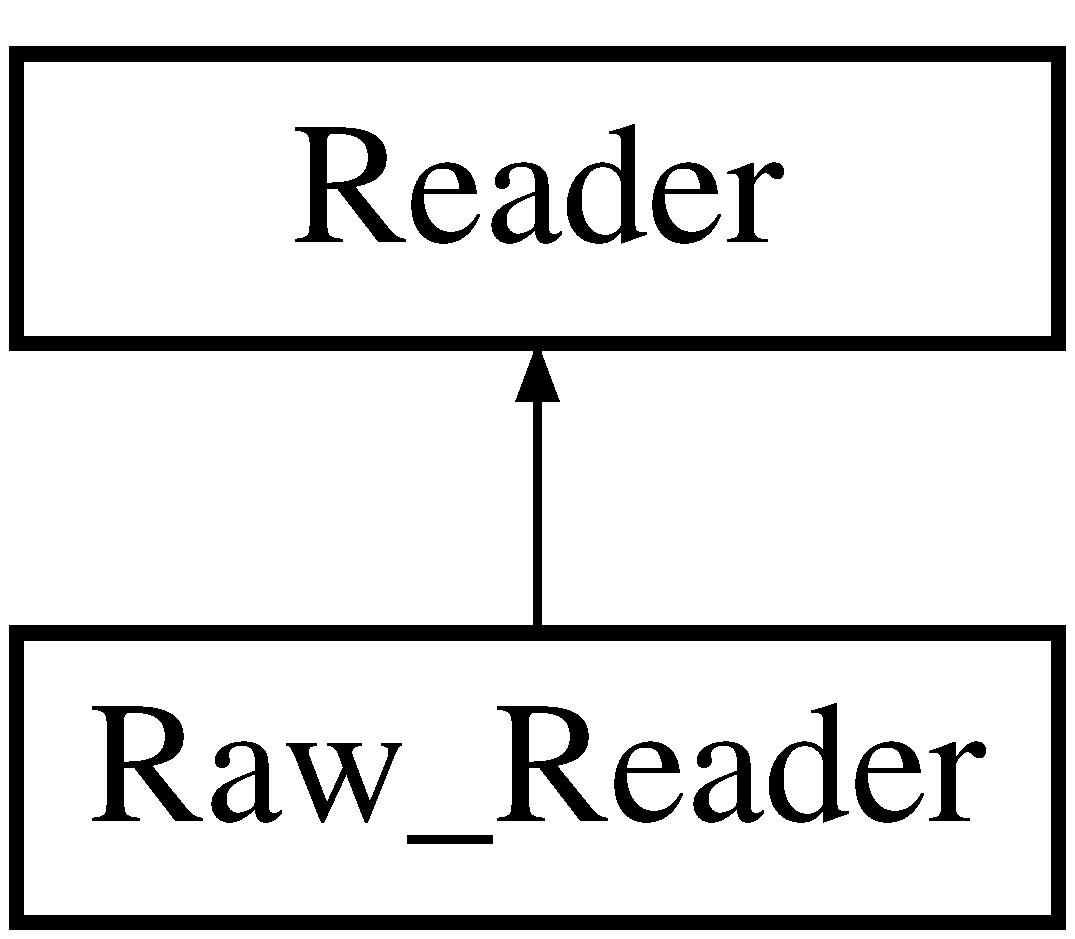
\includegraphics[height=2cm]{classRaw__Reader}
\end{center}
\end{figure}
\subsection*{Public Member Functions}
\begin{DoxyCompactItemize}
\item 
\hyperlink{classRaw__Reader_ae75aca0f781eca8af23e5ac27fa89aae}{Raw\_\-Reader} (const char $\ast$name)
\item 
virtual void \hyperlink{classRaw__Reader_a135e1dd4eadb2afaf201002d5402f21e}{LoadForStaticAnalise} (char $\ast$\&buf, unsigned int \&len, unsigned int \&start)
\item 
virtual void \hyperlink{classRaw__Reader_a9e9a6cafa1b830d5c05b7a5e720c656c}{LoadForDynamicAnalise} (char $\ast$\&buf, unsigned int \&len, unsigned int \&start, unsigned int \&base, unsigned int \&offset)
\item 
virtual \hyperlink{classRaw__Reader_a146ea047af0f0319ada57c5e5768992e}{$\sim$Raw\_\-Reader} ()
\end{DoxyCompactItemize}


\subsection{Detailed Description}
Reads file in $\ast$.Raw format. Format is used in network traffic search. 

\subsection{Constructor \& Destructor Documentation}
\hypertarget{classRaw__Reader_ae75aca0f781eca8af23e5ac27fa89aae}{
\index{Raw\_\-Reader@{Raw\_\-Reader}!Raw\_\-Reader@{Raw\_\-Reader}}
\index{Raw\_\-Reader@{Raw\_\-Reader}!Raw_Reader@{Raw\_\-Reader}}
\subsubsection[{Raw\_\-Reader}]{\setlength{\rightskip}{0pt plus 5cm}Raw\_\-Reader::Raw\_\-Reader (const char $\ast$ {\em name})}}
\label{classRaw__Reader_ae75aca0f781eca8af23e5ac27fa89aae}
Constructor 
\begin{DoxyParams}{Parameters}
\item[{\em name}]file name \end{DoxyParams}
\hypertarget{classRaw__Reader_a146ea047af0f0319ada57c5e5768992e}{
\index{Raw\_\-Reader@{Raw\_\-Reader}!$\sim$Raw\_\-Reader@{$\sim$Raw\_\-Reader}}
\index{$\sim$Raw\_\-Reader@{$\sim$Raw\_\-Reader}!Raw_Reader@{Raw\_\-Reader}}
\subsubsection[{$\sim$Raw\_\-Reader}]{\setlength{\rightskip}{0pt plus 5cm}Raw\_\-Reader::$\sim$Raw\_\-Reader ()\hspace{0.3cm}{\ttfamily  \mbox{[}virtual\mbox{]}}}}
\label{classRaw__Reader_a146ea047af0f0319ada57c5e5768992e}
Destructor 

\subsection{Member Function Documentation}
\hypertarget{classRaw__Reader_a9e9a6cafa1b830d5c05b7a5e720c656c}{
\index{Raw\_\-Reader@{Raw\_\-Reader}!LoadForDynamicAnalise@{LoadForDynamicAnalise}}
\index{LoadForDynamicAnalise@{LoadForDynamicAnalise}!Raw_Reader@{Raw\_\-Reader}}
\subsubsection[{LoadForDynamicAnalise}]{\setlength{\rightskip}{0pt plus 5cm}void Raw\_\-Reader::LoadForDynamicAnalise (char $\ast$\& {\em buf}, \/  unsigned int \& {\em len}, \/  unsigned int \& {\em start}, \/  unsigned int \& {\em base}, \/  unsigned int \& {\em offset})\hspace{0.3cm}{\ttfamily  \mbox{[}virtual\mbox{]}}}}
\label{classRaw__Reader_a9e9a6cafa1b830d5c05b7a5e720c656c}
Load entire file in buffer for Dynamic Analise 
\begin{DoxyParams}{Parameters}
\item[{\em buf}]buffer \item[{\em len}]buffer size \item[{\em start}]entry point =0 in network traffic search \item[{\em base}]is 0x20000000L \item[{\em offset}]is 0 in network traffic search \end{DoxyParams}


Implements \hyperlink{classReader_a0fe4ac206880263e042c5277370c679b}{Reader}.

\hypertarget{classRaw__Reader_a135e1dd4eadb2afaf201002d5402f21e}{
\index{Raw\_\-Reader@{Raw\_\-Reader}!LoadForStaticAnalise@{LoadForStaticAnalise}}
\index{LoadForStaticAnalise@{LoadForStaticAnalise}!Raw_Reader@{Raw\_\-Reader}}
\subsubsection[{LoadForStaticAnalise}]{\setlength{\rightskip}{0pt plus 5cm}void Raw\_\-Reader::LoadForStaticAnalise (char $\ast$\& {\em buf}, \/  unsigned int \& {\em len}, \/  unsigned int \& {\em start})\hspace{0.3cm}{\ttfamily  \mbox{[}virtual\mbox{]}}}}
\label{classRaw__Reader_a135e1dd4eadb2afaf201002d5402f21e}
Load entire file in buffer for Static Analise 
\begin{DoxyParams}{Parameters}
\item[{\em buf}]buffer \item[{\em len}]buffer size \item[{\em start}]entry point =0 in network traffic search \end{DoxyParams}


Implements \hyperlink{classReader_a48b1d822c048d481388fe05ff90b10f3}{Reader}.



The documentation for this class was generated from the following files:\begin{DoxyCompactItemize}
\item 
PE\_\-Reader.h\item 
PE\_\-Reader.cpp\end{DoxyCompactItemize}

\hypertarget{classReader}{
\section{Reader Class Reference}
\label{classReader}\index{Reader@{Reader}}
}


{\ttfamily \#include $<$PE\_\-Reader.h$>$}

Inheritance diagram for Reader:\begin{figure}[H]
\begin{center}
\leavevmode
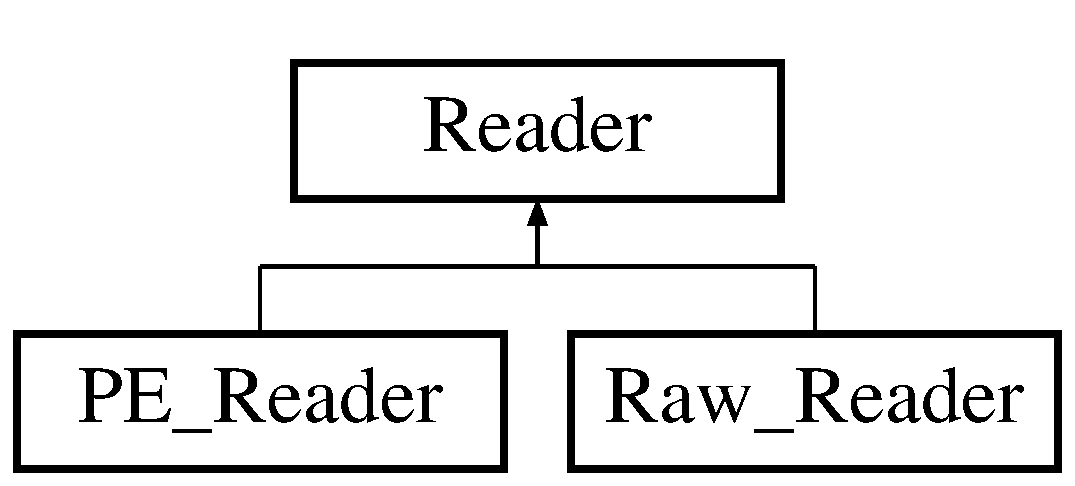
\includegraphics[height=2cm]{classReader}
\end{center}
\end{figure}
\subsection*{Public Member Functions}
\begin{DoxyCompactItemize}
\item 
virtual void \hyperlink{classReader_a48b1d822c048d481388fe05ff90b10f3}{LoadForStaticAnalise} (char $\ast$\&buf, unsigned int \&len, unsigned int \&start)=0
\begin{DoxyCompactList}\small\item\em file pointer \item\end{DoxyCompactList}\item 
virtual void \hyperlink{classReader_a0fe4ac206880263e042c5277370c679b}{LoadForDynamicAnalise} (char $\ast$\&buf, unsigned int \&len, unsigned int \&start, unsigned int \&base, unsigned int \&offset)=0
\end{DoxyCompactItemize}
\subsection*{Protected Attributes}
\begin{DoxyCompactItemize}
\item 
\hypertarget{classReader_a583b5c9cc809c6630c9cade472c6f50e}{
char $\ast$ {\bfseries filename}}
\label{classReader_a583b5c9cc809c6630c9cade472c6f50e}

\item 
\hypertarget{classReader_ad8968e3f303fe580f2ab5077ae8be377}{
FILE $\ast$ \hyperlink{classReader_ad8968e3f303fe580f2ab5077ae8be377}{fp}}
\label{classReader_ad8968e3f303fe580f2ab5077ae8be377}

\begin{DoxyCompactList}\small\item\em name of the input file \item\end{DoxyCompactList}\end{DoxyCompactItemize}


\subsection{Detailed Description}
Abstract class 

\subsection{Member Function Documentation}
\hypertarget{classReader_a0fe4ac206880263e042c5277370c679b}{
\index{Reader@{Reader}!LoadForDynamicAnalise@{LoadForDynamicAnalise}}
\index{LoadForDynamicAnalise@{LoadForDynamicAnalise}!Reader@{Reader}}
\subsubsection[{LoadForDynamicAnalise}]{\setlength{\rightskip}{0pt plus 5cm}virtual void Reader::LoadForDynamicAnalise (char $\ast$\& {\em buf}, \/  unsigned int \& {\em len}, \/  unsigned int \& {\em start}, \/  unsigned int \& {\em base}, \/  unsigned int \& {\em offset})\hspace{0.3cm}{\ttfamily  \mbox{[}pure virtual\mbox{]}}}}
\label{classReader_a0fe4ac206880263e042c5277370c679b}
Load entire file in buffer for Dynamic Analise 
\begin{DoxyParams}{Parameters}
\item[{\em buf}]buffer \item[{\em len}]buffer size \item[{\em start}]entry point \item[{\em base}]base=0x20000000L \item[{\em offset}]\end{DoxyParams}


Implemented in \hyperlink{classRaw__Reader_a9e9a6cafa1b830d5c05b7a5e720c656c}{Raw\_\-Reader}, and \hyperlink{classPE__Reader_ad11f69fdbf231385c9ff7edd26913af7}{PE\_\-Reader}.

\hypertarget{classReader_a48b1d822c048d481388fe05ff90b10f3}{
\index{Reader@{Reader}!LoadForStaticAnalise@{LoadForStaticAnalise}}
\index{LoadForStaticAnalise@{LoadForStaticAnalise}!Reader@{Reader}}
\subsubsection[{LoadForStaticAnalise}]{\setlength{\rightskip}{0pt plus 5cm}virtual void Reader::LoadForStaticAnalise (char $\ast$\& {\em buf}, \/  unsigned int \& {\em len}, \/  unsigned int \& {\em start})\hspace{0.3cm}{\ttfamily  \mbox{[}pure virtual\mbox{]}}}}
\label{classReader_a48b1d822c048d481388fe05ff90b10f3}


file pointer 

Load file in buffer for Static Analise 
\begin{DoxyParams}{Parameters}
\item[{\em buf}]buffer \item[{\em len}]buffer size \item[{\em start}]entry point =0 in network traffic search \end{DoxyParams}


Implemented in \hyperlink{classRaw__Reader_a135e1dd4eadb2afaf201002d5402f21e}{Raw\_\-Reader}, and \hyperlink{classPE__Reader_a4b5e1c738c887247181c4e3d0f253c27}{PE\_\-Reader}.



The documentation for this class was generated from the following file:\begin{DoxyCompactItemize}
\item 
PE\_\-Reader.h\end{DoxyCompactItemize}

\hypertarget{classStack}{
\section{Stack Class Reference}
\label{classStack}\index{Stack@{Stack}}
}
\subsection*{Public Member Functions}
\begin{DoxyCompactItemize}
\item 
\hyperlink{classStack_a14cd1cba325bead4ff0a91bc6eb0f6f5}{Stack} ()
\begin{DoxyCompactList}\small\item\em first address in \hyperlink{classStack}{Stack} \item\end{DoxyCompactList}\item 
void \hyperlink{classStack_af37f0135217037f2015513f984344e7b}{Push} (const unsigned int a)
\item 
void \hyperlink{classStack_a5f548c0c416082bba3c14e34752a3d0c}{Pop} (unsigned int \&a)
\item 
void \hyperlink{classStack_a2f06e658c01857727857ee5499b2e465}{Print} ()
\item 
\hyperlink{classStack_a40bd5dff912f0e5290777c4b46d17809}{$\sim$Stack} ()
\end{DoxyCompactItemize}


\subsection{Constructor \& Destructor Documentation}
\hypertarget{classStack_a14cd1cba325bead4ff0a91bc6eb0f6f5}{
\index{Stack@{Stack}!Stack@{Stack}}
\index{Stack@{Stack}!Stack@{Stack}}
\subsubsection[{Stack}]{\setlength{\rightskip}{0pt plus 5cm}Stack::Stack ()}}
\label{classStack_a14cd1cba325bead4ff0a91bc6eb0f6f5}


first address in \hyperlink{classStack}{Stack} 

default constructor \hypertarget{classStack_a40bd5dff912f0e5290777c4b46d17809}{
\index{Stack@{Stack}!$\sim$Stack@{$\sim$Stack}}
\index{$\sim$Stack@{$\sim$Stack}!Stack@{Stack}}
\subsubsection[{$\sim$Stack}]{\setlength{\rightskip}{0pt plus 5cm}Stack::$\sim$Stack ()}}
\label{classStack_a40bd5dff912f0e5290777c4b46d17809}
default destructor 

\subsection{Member Function Documentation}
\hypertarget{classStack_a5f548c0c416082bba3c14e34752a3d0c}{
\index{Stack@{Stack}!Pop@{Pop}}
\index{Pop@{Pop}!Stack@{Stack}}
\subsubsection[{Pop}]{\setlength{\rightskip}{0pt plus 5cm}void Stack::Pop (unsigned int \& {\em a})}}
\label{classStack_a5f548c0c416082bba3c14e34752a3d0c}
Pops next address from \hyperlink{classStack}{Stack} 
\begin{DoxyParams}{Parameters}
\item[{\em a}]address \end{DoxyParams}
\hypertarget{classStack_a2f06e658c01857727857ee5499b2e465}{
\index{Stack@{Stack}!Print@{Print}}
\index{Print@{Print}!Stack@{Stack}}
\subsubsection[{Print}]{\setlength{\rightskip}{0pt plus 5cm}void Stack::Print ()}}
\label{classStack_a2f06e658c01857727857ee5499b2e465}
Prints all addresses in stack \hypertarget{classStack_af37f0135217037f2015513f984344e7b}{
\index{Stack@{Stack}!Push@{Push}}
\index{Push@{Push}!Stack@{Stack}}
\subsubsection[{Push}]{\setlength{\rightskip}{0pt plus 5cm}void Stack::Push (const unsigned int {\em a})}}
\label{classStack_af37f0135217037f2015513f984344e7b}
Pushes next address in \hyperlink{classStack}{Stack} 
\begin{DoxyParams}{Parameters}
\item[{\em a}]address \end{DoxyParams}


The documentation for this class was generated from the following files:\begin{DoxyCompactItemize}
\item 
Stack.h\item 
Stack.cpp\end{DoxyCompactItemize}

\hypertarget{structUsed}{
\section{Used Struct Reference}
\label{structUsed}\index{Used@{Used}}
}


\subsection{Detailed Description}
node/leaf in class \hyperlink{classInstruction__Tree}{Instruction\_\-Tree}. 

The documentation for this struct was generated from the following file:\begin{DoxyCompactItemize}
\item 
Instruction\_\-Leaf.h\end{DoxyCompactItemize}

\printindex
\end{document}
